\documentclass{article}

\usepackage[utf8]{inputenc}
\usepackage[bottom=2cm, top=2cm, left=2cm, right=2cm]{geometry}
\usepackage{verbatim}
\usepackage{tikz}
\usetikzlibrary{chains}

\title{Lista 7}
\author{Vinícius Couto Tasso}
\date{}

\begin{document}

\maketitle
\tikzset{every tree node/.style={minimum width=2em,draw,circle},
         blank/.style={draw=none},
         edge from parent/.style=
         {draw,edge from parent path={(\tikzparentnode) -- (\tikzchildnode)}},
         level distance=1cm}
         
\begin{enumerate}

\setcounter{enumi}{1}

\item \textbf{A sequência $\langle 23, 17, 14, 6, 13, 10, 1, 5, 7, 12 \rangle$ é um heap máximo?}

Não, pois o nó de valor 7 é maior que seu pai, de valor 6.

\item \textbf{Ilustre a operação \texttt{MAX-HEAPIFY(V,3)} sobre o arranjo $V = \langle 23, 17, 3, 16, 13, 10, 1, 5, 7, 12, 4, 8, 9, 0 \rangle$.}


\begin{center}
    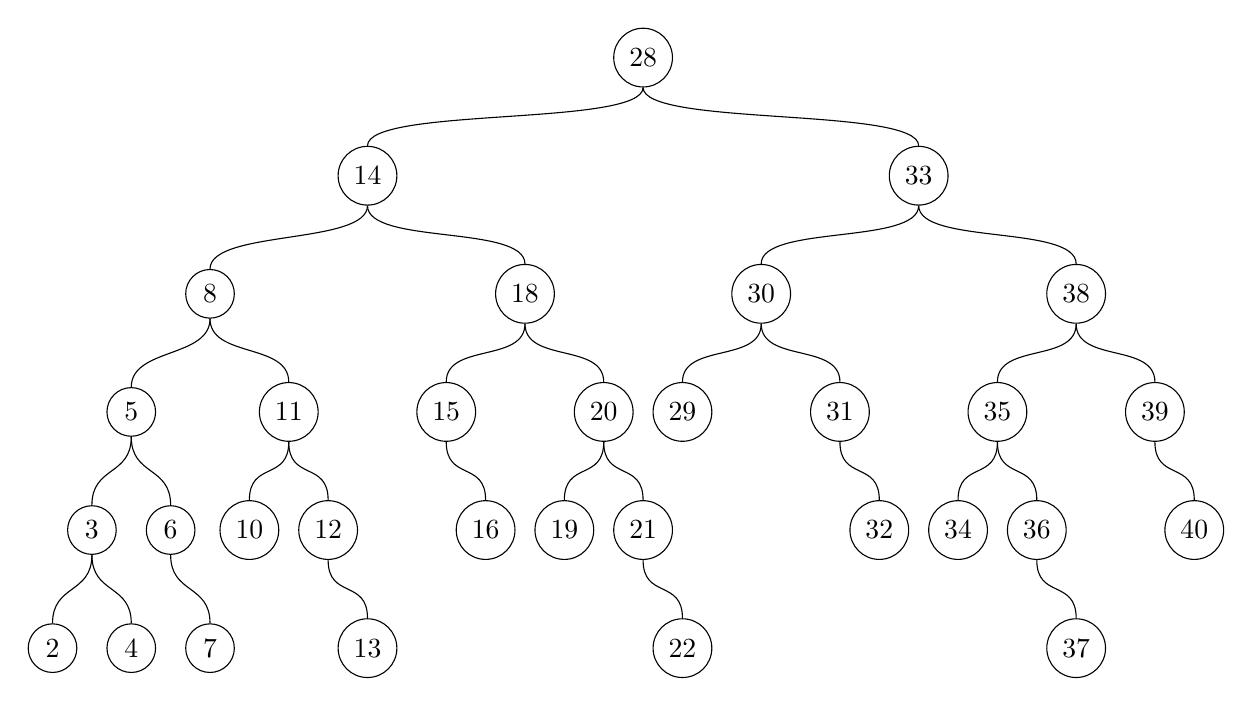
\begin{tikzpicture}[
       edge from parent path=
    {(\tikzparentnode.south) .. controls +(0,-.5) and +(0,.5)
                             .. (\tikzchildnode.north)},
    level 1/.style={sibling distance=7cm},                        
    level 2/.style={sibling distance=4cm},                         
    level 3/.style={sibling distance=2cm},
    level 4/.style={sibling distance=1cm},
   every node/.style={draw,circle},
   label distance=-1mm]
   
\node {28}
    child {node {14}
        child {node {8}
            child {node {5}
                child {node {3}
                    child {node {2}}
                    child {node {4}}
                }
                child {node {6}
                    child[missing] {}
                    child {node {7}}
                }
            }
            child {node {11}
                child {node {10}}
                child {node {12}
                    child[missing] {}   
                    child {node {13}}
                }
            }
        }
        child {node {18}
            child {node {15}
                child[missing] {}   
                child {node {16}}
            }
            child {node {20}
                child {node {19}}
                child {node {21}
                    child[missing] {}   
                    child {node {22}}
                }
            }
        }
    }   
    child {node {33}
        child {node {30}
            child {node {29}}
            child {node {31}
                    child[missing] {}
                    child {node {32}}
                }
            }
        child {node {38}
            child {node {35}
                child {node {34}}
                child {node {36}
                    child[missing] {}
                    child {node {37}}
                }
            }
            child {node {39}
                child[missing] {}
                child {node {40}}
            }
        }
    };

\end{tikzpicture}
\end{center}

\newpage

\item \textbf{Ilustre a operação \texttt{BUILD-MAX-HEAP} sobre o arranjo $V = \langle 5, 3, 17, 10, 84, 19, 6, 22, 9 \rangle$.}

\begin{center}
    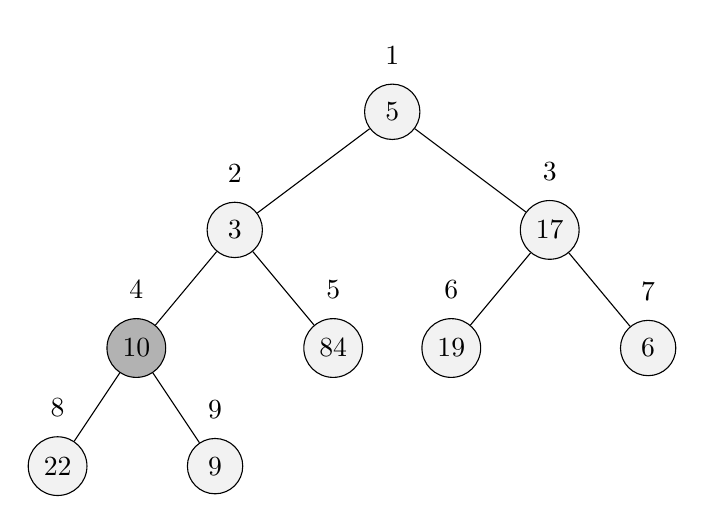
\begin{tikzpicture}
   \tikzstyle{level 1}=[sibling distance=4cm]
   \tikzstyle{level 2}=[sibling distance=2.5cm]
   \tikzstyle{level 3}=[sibling distance=2cm]
   \tikzstyle{every node}=[draw, circle, fill=gray, fill opacity=0.1, text opacity=1, minimum size=2em]
   
\node[label=90:$1$] {5}
    child {node[label=90:$2$] {3}
        child {node[label=90:$4$, fill=black, fill opacity=0.3] {10}
            child {node[label=90:$8$] {22}}
            child {node[label=90:$9$] {9}}
        }
        child {node[label=90:$5$] {84}}
    }
    child {node[label=90:$3$] {17}
        child {node[label=90:$6$] {19}}
        child {node[label=90:$7$] {6}}
    };

\end{tikzpicture}
\end{center}

\begin{center}
    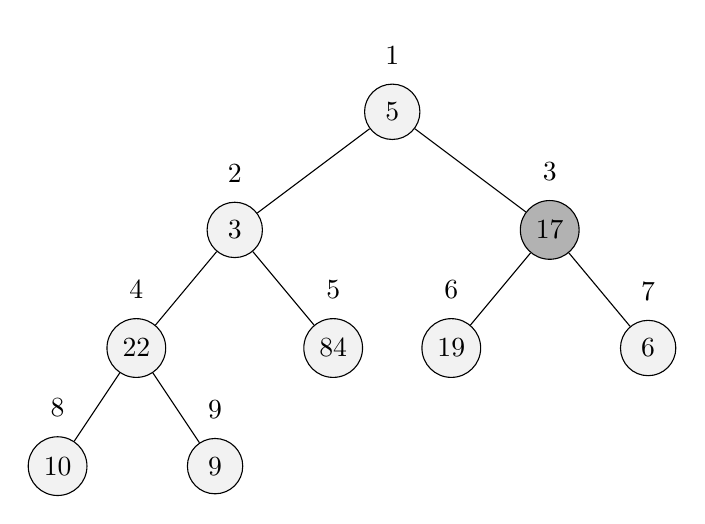
\begin{tikzpicture}
   \tikzstyle{level 1}=[sibling distance=4cm]
   \tikzstyle{level 2}=[sibling distance=2.5cm]
   \tikzstyle{level 3}=[sibling distance=2cm]
   \tikzstyle{every node}=[draw, circle, fill=gray, fill opacity=0.1, text opacity=1, minimum size=2em]
   
\node[label=90:$1$] {5}
    child {node[label=90:$2$] {3}
        child {node[label=90:$4$] {22}
            child {node[label=90:$8$] {10}}
            child {node[label=90:$9$] {9}}
        }
        child {node[label=90:$5$] {84}}
    }
    child {node[label=90:$3$, fill=black, fill opacity=0.3] {17}
        child {node[label=90:$6$] {19}}
        child {node[label=90:$7$] {6}}
    };

\end{tikzpicture}
\end{center}

\begin{center}
    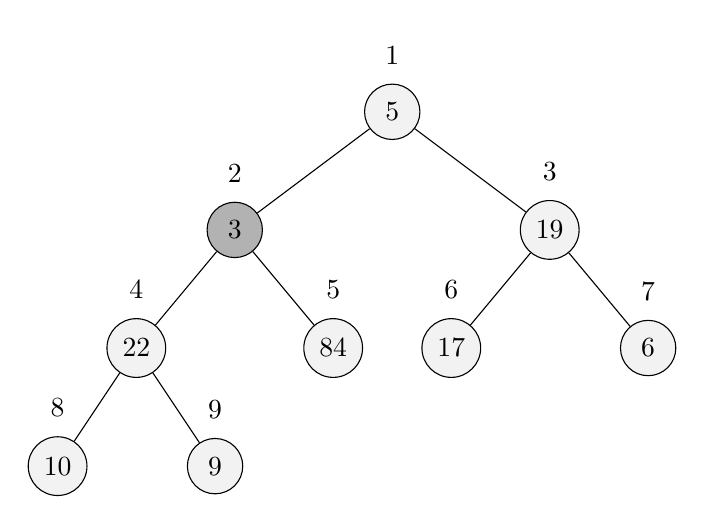
\begin{tikzpicture}
   \tikzstyle{level 1}=[sibling distance=4cm]
   \tikzstyle{level 2}=[sibling distance=2.5cm]
   \tikzstyle{level 3}=[sibling distance=2cm]
   \tikzstyle{every node}=[draw, circle, fill=gray, fill opacity=0.1, text opacity=1, minimum size=2em]
   
\node[label=90:$1$] {5}
    child {node[label=90:$2$, fill=black, fill opacity=0.3] {3}
        child {node[label=90:$4$] {22}
            child {node[label=90:$8$] {10}}
            child {node[label=90:$9$] {9}}
        }
        child {node[label=90:$5$] {84}}
    }
    child {node[label=90:$3$] {19}
        child {node[label=90:$6$] {17}}
        child {node[label=90:$7$] {6}}
    };

\end{tikzpicture}
\end{center}

\begin{center}
    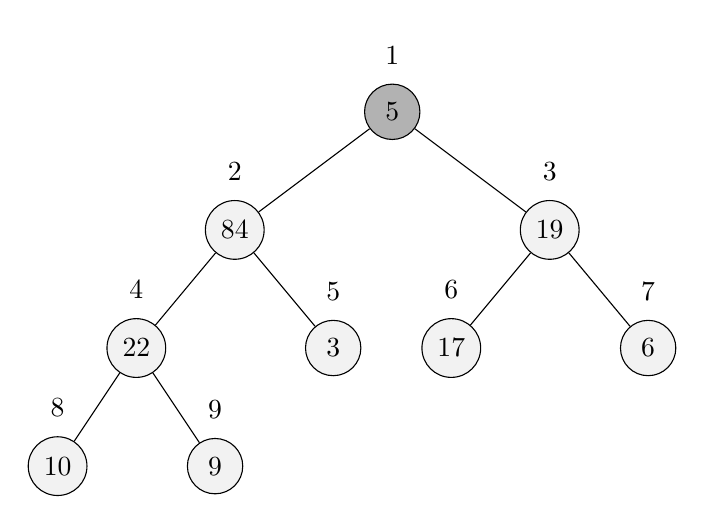
\begin{tikzpicture}
   \tikzstyle{level 1}=[sibling distance=4cm]
   \tikzstyle{level 2}=[sibling distance=2.5cm]
   \tikzstyle{level 3}=[sibling distance=2cm]
   \tikzstyle{every node}=[draw, circle, fill=gray, fill opacity=0.1, text opacity=1, minimum size=2em]
   
\node[label=90:$1$, fill=black, fill opacity=0.3] {5}
    child {node[label=90:$2$] {84}
        child {node[label=90:$4$] {22}
            child {node[label=90:$8$] {10}}
            child {node[label=90:$9$] {9}}
        }
        child {node[label=90:$5$] {3}}
    }
    child {node[label=90:$3$] {19}
        child {node[label=90:$6$] {17}}
        child {node[label=90:$7$] {6}}
    };

\end{tikzpicture}
\end{center}

\begin{center}
    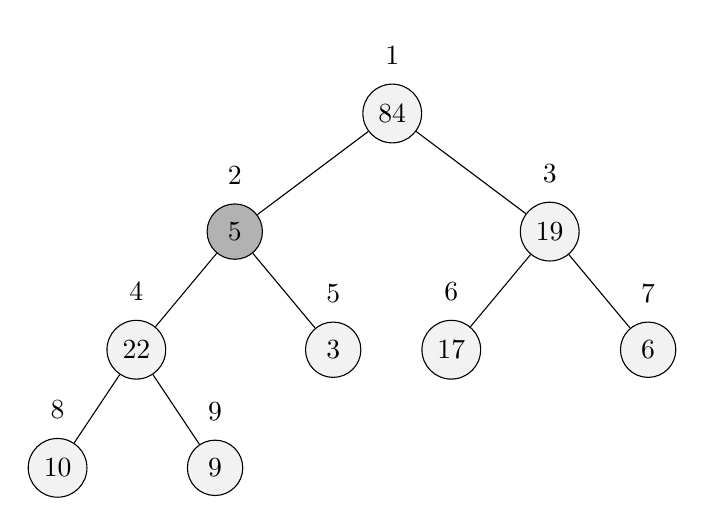
\begin{tikzpicture}
   \tikzstyle{level 1}=[sibling distance=4cm]
   \tikzstyle{level 2}=[sibling distance=2.5cm]
   \tikzstyle{level 3}=[sibling distance=2cm]
   \tikzstyle{every node}=[draw, circle, fill=gray, fill opacity=0.1, text opacity=1, minimum size=2em]
   
\node[label=90:$1$] {84}
    child {node[label=90:$2$, fill=black, fill opacity=0.3] {5}
        child {node[label=90:$4$] {22}
            child {node[label=90:$8$] {10}}
            child {node[label=90:$9$] {9}}
        }
        child {node[label=90:$5$] {3}}
    }
    child {node[label=90:$3$] {19}
        child {node[label=90:$6$] {17}}
        child {node[label=90:$7$] {6}}
    };

\end{tikzpicture}
\end{center}

\begin{center}
    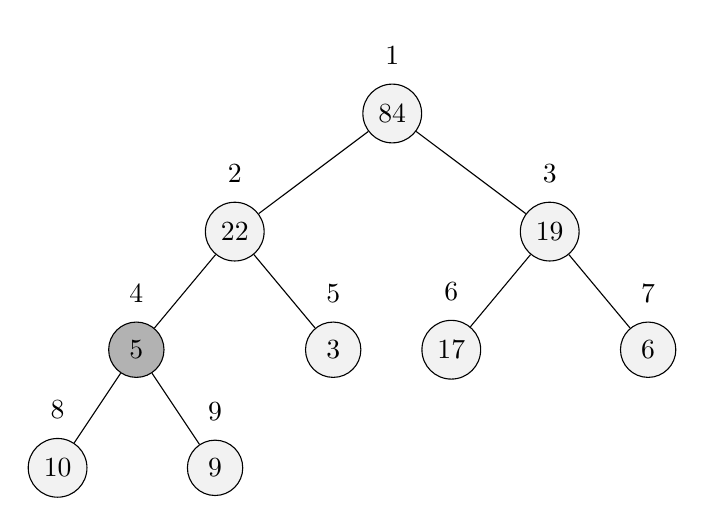
\begin{tikzpicture}
   \tikzstyle{level 1}=[sibling distance=4cm]
   \tikzstyle{level 2}=[sibling distance=2.5cm]
   \tikzstyle{level 3}=[sibling distance=2cm]
   \tikzstyle{every node}=[draw, circle, fill=gray, fill opacity=0.1, text opacity=1, minimum size=2em]
   
\node[label=90:$1$] {84}
    child {node[label=90:$2$] {22}
        child {node[label=90:$4$, fill=black, fill opacity=0.3] {5}
            child {node[label=90:$8$] {10}}
            child {node[label=90:$9$] {9}}
        }
        child {node[label=90:$5$] {3}}
    }
    child {node[label=90:$3$] {19}
        child {node[label=90:$6$] {17}}
        child {node[label=90:$7$] {6}}
    };

\end{tikzpicture}
\end{center}

\begin{center}
    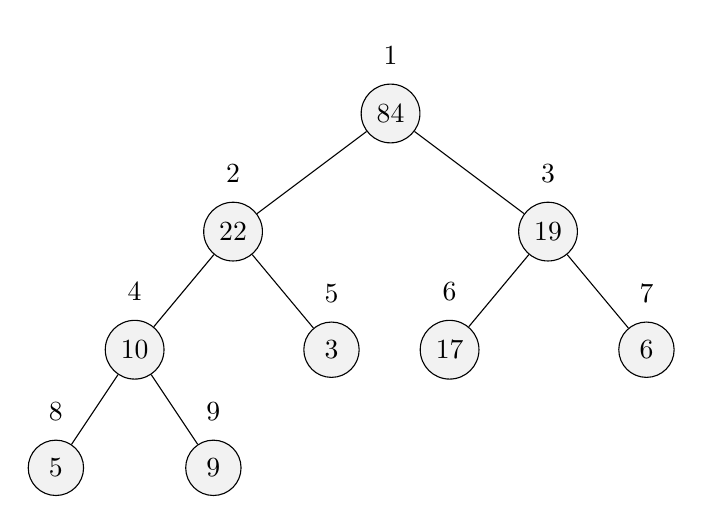
\begin{tikzpicture}
   \tikzstyle{level 1}=[sibling distance=4cm]
   \tikzstyle{level 2}=[sibling distance=2.5cm]
   \tikzstyle{level 3}=[sibling distance=2cm]
   \tikzstyle{every node}=[draw, circle, fill=gray, fill opacity=0.1, text opacity=1, minimum size=2em]
   
\node[label=90:$1$] {84}
    child {node[label=90:$2$] {22}
        child {node[label=90:$4$] {10}
            child {node[label=90:$8$] {5}}
            child {node[label=90:$9$] {9}}
        }
        child {node[label=90:$5$] {3}}
    }
    child {node[label=90:$3$] {19}
        child {node[label=90:$6$] {17}}
        child {node[label=90:$7$] {6}}
    };

\end{tikzpicture}
\end{center}

\item \textbf{Ilustre a operação \texttt{HEAP-SORT} sobre o arranjo $V = \langle 5, 13, 2, 25, 7, 17, 20, 8, 4 \rangle$.}

\begin{center}
    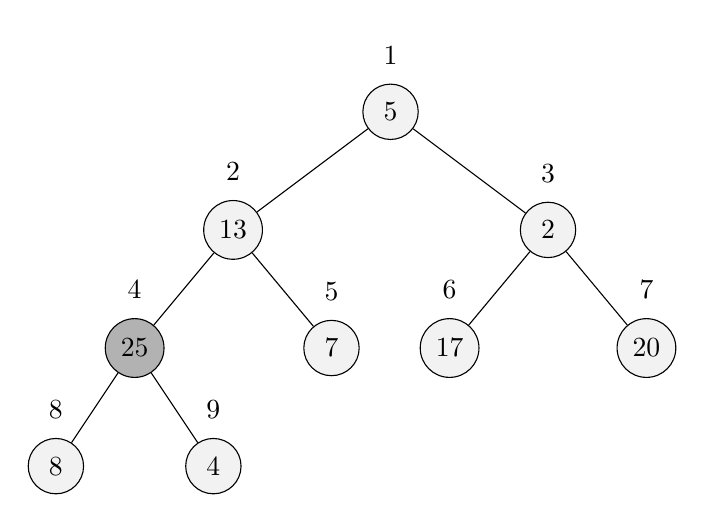
\begin{tikzpicture}
   \tikzstyle{level 1}=[sibling distance=4cm]
   \tikzstyle{level 2}=[sibling distance=2.5cm]
   \tikzstyle{level 3}=[sibling distance=2cm]
   \tikzstyle{every node}=[draw, circle, fill=gray, fill opacity=0.1, text opacity=1, minimum size=2em]
   
\node[label=90:$1$] {5}
    child {node[label=90:$2$] {13}
        child {node[label=90:$4$, fill=black, fill opacity=0.3] {25}
            child {node[label=90:$8$] {8}}
            child {node[label=90:$9$] {4}}
        }
        child {node[label=90:$5$] {7}}
    }
    child {node[label=90:$3$] {2}
        child {node[label=90:$6$] {17}}
        child {node[label=90:$7$] {20}}
    };

\end{tikzpicture}
\end{center}

\begin{center}
    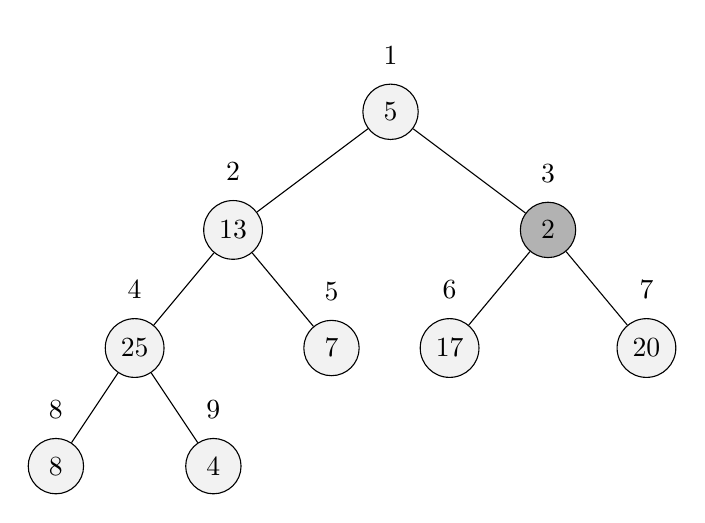
\begin{tikzpicture}
   \tikzstyle{level 1}=[sibling distance=4cm]
   \tikzstyle{level 2}=[sibling distance=2.5cm]
   \tikzstyle{level 3}=[sibling distance=2cm]
   \tikzstyle{every node}=[draw, circle, fill=gray, fill opacity=0.1, text opacity=1, minimum size=2em]
   
\node[label=90:$1$] {5}
    child {node[label=90:$2$] {13}
        child {node[label=90:$4$] {25}
            child {node[label=90:$8$] {8}}
            child {node[label=90:$9$] {4}}
        }
        child {node[label=90:$5$] {7}}
    }
    child {node[label=90:$3$, fill=black, fill opacity=0.3] {2}
        child {node[label=90:$6$] {17}}
        child {node[label=90:$7$] {20}}
    };

\end{tikzpicture}
\end{center}

\begin{center}
    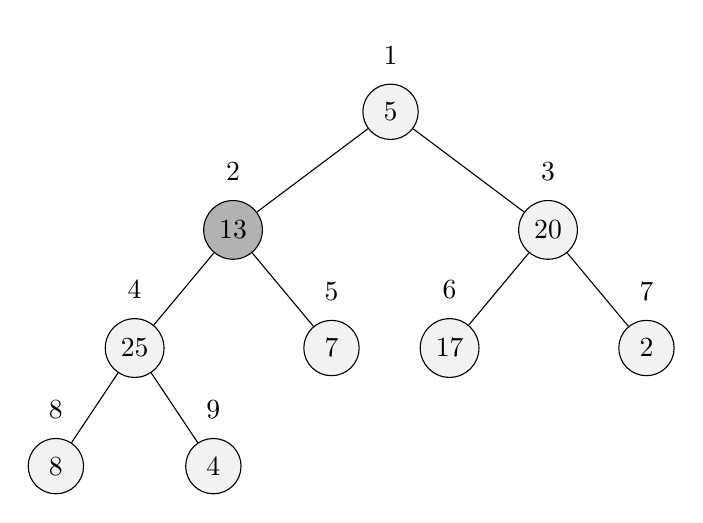
\begin{tikzpicture}
   \tikzstyle{level 1}=[sibling distance=4cm]
   \tikzstyle{level 2}=[sibling distance=2.5cm]
   \tikzstyle{level 3}=[sibling distance=2cm]
   \tikzstyle{every node}=[draw, circle, fill=gray, fill opacity=0.1, text opacity=1, minimum size=2em]
   
\node[label=90:$1$] {5}
    child {node[label=90:$2$, fill=black, fill opacity=0.3] {13}
        child {node[label=90:$4$] {25}
            child {node[label=90:$8$] {8}}
            child {node[label=90:$9$] {4}}
        }
        child {node[label=90:$5$] {7}}
    }
    child {node[label=90:$3$] {20}
        child {node[label=90:$6$] {17}}
        child {node[label=90:$7$] {2}}
    };

\end{tikzpicture}
\end{center}

\begin{center}
    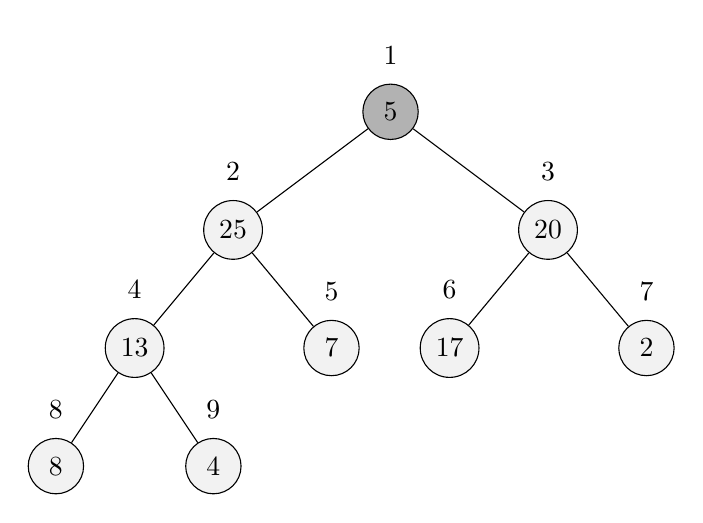
\begin{tikzpicture}
   \tikzstyle{level 1}=[sibling distance=4cm]
   \tikzstyle{level 2}=[sibling distance=2.5cm]
   \tikzstyle{level 3}=[sibling distance=2cm]
   \tikzstyle{every node}=[draw, circle, fill=gray, fill opacity=0.1, text opacity=1, minimum size=2em]
   
\node[label=90:$1$, fill=black, fill opacity=0.3] {5}
    child {node[label=90:$2$] {25}
        child {node[label=90:$4$] {13}
            child {node[label=90:$8$] {8}}
            child {node[label=90:$9$] {4}}
        }
        child {node[label=90:$5$] {7}}
    }
    child {node[label=90:$3$] {20}
        child {node[label=90:$6$] {17}}
        child {node[label=90:$7$] {2}}
    };

\end{tikzpicture}
\end{center}

\begin{center}
    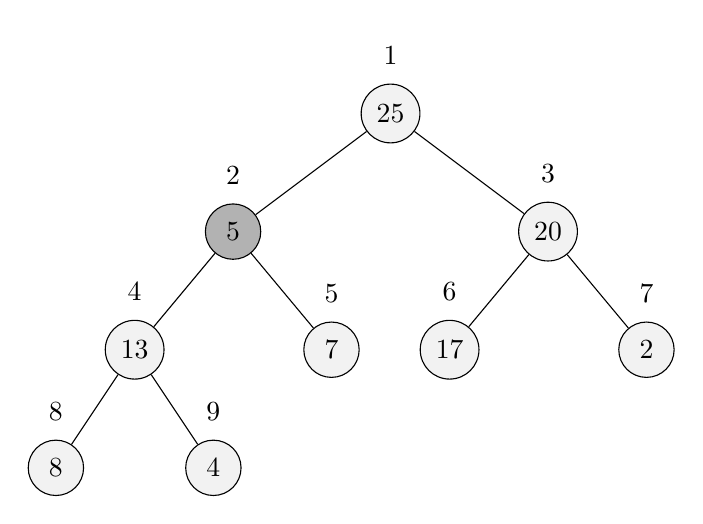
\begin{tikzpicture}
   \tikzstyle{level 1}=[sibling distance=4cm]
   \tikzstyle{level 2}=[sibling distance=2.5cm]
   \tikzstyle{level 3}=[sibling distance=2cm]
   \tikzstyle{every node}=[draw, circle, fill=gray, fill opacity=0.1, text opacity=1, minimum size=2em]
   
\node[label=90:$1$] {25}
    child {node[label=90:$2$, fill=black, fill opacity=0.3] {5}
        child {node[label=90:$4$] {13}
            child {node[label=90:$8$] {8}}
            child {node[label=90:$9$] {4}}
        }
        child {node[label=90:$5$] {7}}
    }
    child {node[label=90:$3$] {20}
        child {node[label=90:$6$] {17}}
        child {node[label=90:$7$] {2}}
    };

\end{tikzpicture}
\end{center}

\begin{center}
    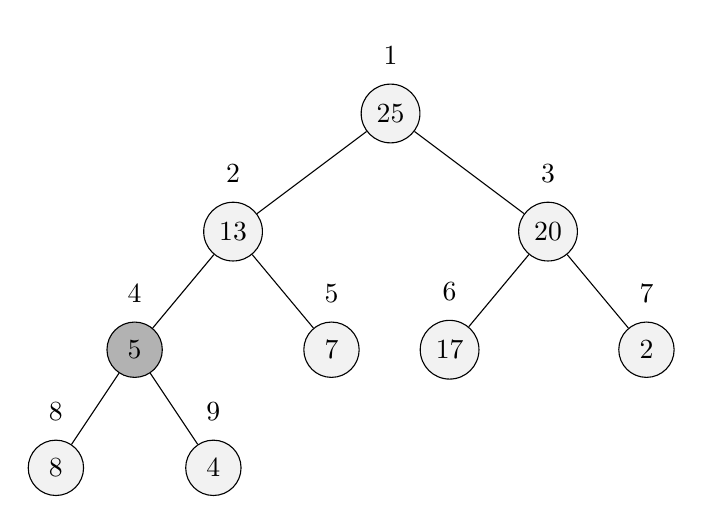
\begin{tikzpicture}
   \tikzstyle{level 1}=[sibling distance=4cm]
   \tikzstyle{level 2}=[sibling distance=2.5cm]
   \tikzstyle{level 3}=[sibling distance=2cm]
   \tikzstyle{every node}=[draw, circle, fill=gray, fill opacity=0.1, text opacity=1, minimum size=2em]
   
\node[label=90:$1$] {25}
    child {node[label=90:$2$] {13}
        child {node[label=90:$4$, fill=black, fill opacity=0.3] {5}
            child {node[label=90:$8$] {8}}
            child {node[label=90:$9$] {4}}
        }
        child {node[label=90:$5$] {7}}
    }
    child {node[label=90:$3$] {20}
        child {node[label=90:$6$] {17}}
        child {node[label=90:$7$] {2}}
    };

\end{tikzpicture}
\end{center}

\begin{center}
    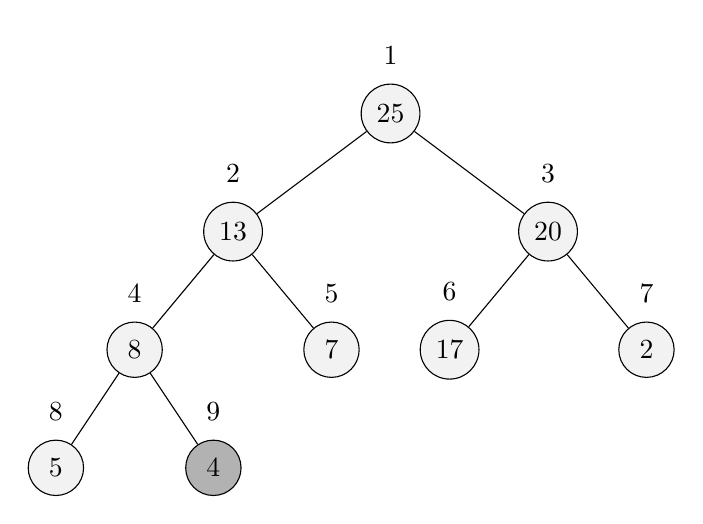
\begin{tikzpicture}
   \tikzstyle{level 1}=[sibling distance=4cm]
   \tikzstyle{level 2}=[sibling distance=2.5cm]
   \tikzstyle{level 3}=[sibling distance=2cm]
   \tikzstyle{every node}=[draw, circle, fill=gray, fill opacity=0.1, text opacity=1, minimum size=2em]
   
\node[label=90:$1$] {25}
    child {node[label=90:$2$] {13}
        child {node[label=90:$4$] {8}
            child {node[label=90:$8$] {5}}
            child {node[label=90:$9$, fill=black, fill opacity=0.3] {4}}
        }
        child {node[label=90:$5$] {7}}
    }
    child {node[label=90:$3$] {20}
        child {node[label=90:$6$] {17}}
        child {node[label=90:$7$] {2}}
    };

\end{tikzpicture}
\end{center}

% Start heapsort

\begin{center}
    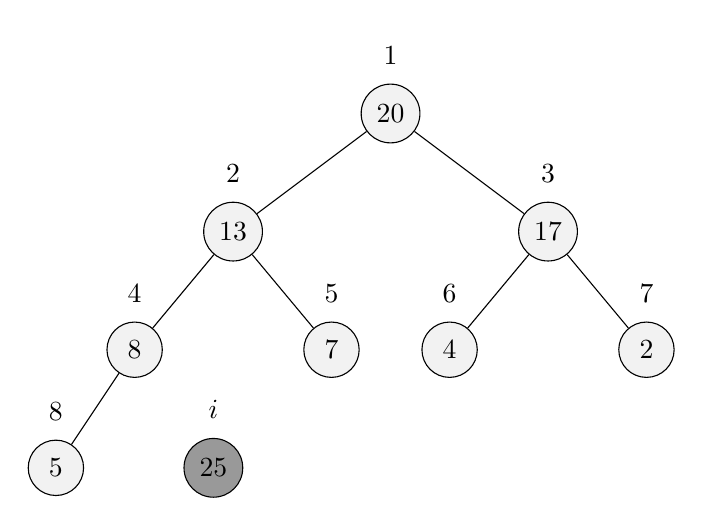
\begin{tikzpicture}
   \tikzstyle{level 1}=[sibling distance=4cm]
   \tikzstyle{level 2}=[sibling distance=2.5cm]
   \tikzstyle{level 3}=[sibling distance=2cm]
   \tikzstyle{every node}=[draw, circle, fill=gray, fill opacity=0.1, text opacity=1, minimum size=2em]
   
\node[label=90:$1$] {20}
    child {node[label=90:$2$] {13}
        child {node[label=90:$4$] {8}
            child {node[label=90:$8$] {5}}
            child {node[label=90:$i$, fill=black, fill opacity=0.4] {25} edge from parent[draw=none]}
        }
        child {node[label=90:$5$] {7}}
    }
    child {node[label=90:$3$] {17}
        child {node[label=90:$6$] {4}}
        child {node[label=90:$7$] {2}}
    };

\end{tikzpicture}
\end{center}

\begin{center}
    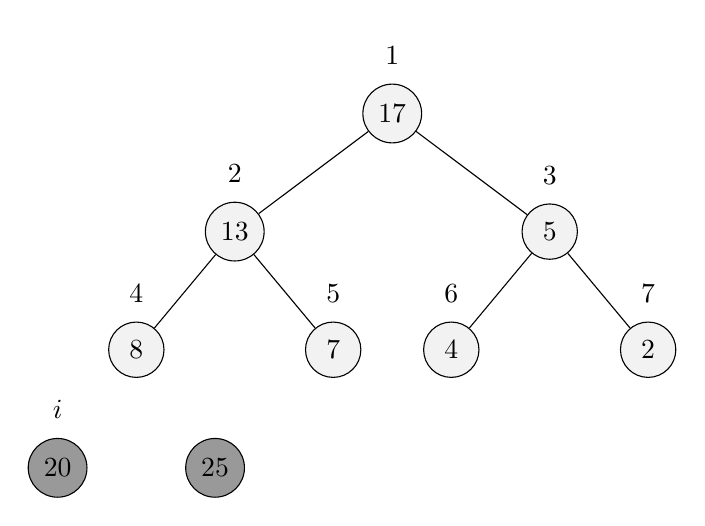
\begin{tikzpicture}
   \tikzstyle{level 1}=[sibling distance=4cm]
   \tikzstyle{level 2}=[sibling distance=2.5cm]
   \tikzstyle{level 3}=[sibling distance=2cm]
   \tikzstyle{every node}=[draw, circle, fill=gray, fill opacity=0.1, text opacity=1, minimum size=2em]
   
\node[label=90:$1$] {17}
    child {node[label=90:$2$] {13}
        child {node[label=90:$4$] {8}
            child {node[label=90:$i$, fill=black, fill opacity=0.4] {20} edge from parent[draw=none]}
            child {node[fill=black, fill opacity=0.4] {25} edge from parent[draw=none]}
        }
        child {node[label=90:$5$] {7}}
    }
    child {node[label=90:$3$] {5}
        child {node[label=90:$6$] {4}}
        child {node[label=90:$7$] {2}}
    };

\end{tikzpicture}
\end{center}

\begin{center}
    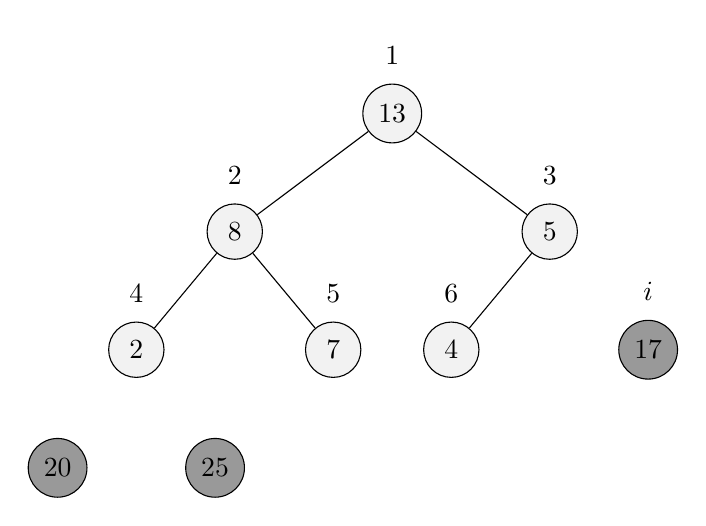
\begin{tikzpicture}
   \tikzstyle{level 1}=[sibling distance=4cm]
   \tikzstyle{level 2}=[sibling distance=2.5cm]
   \tikzstyle{level 3}=[sibling distance=2cm]
   \tikzstyle{every node}=[draw, circle, fill=gray, fill opacity=0.1, text opacity=1, minimum size=2em]
   
\node[label=90:$1$] {13}
    child {node[label=90:$2$] {8}
        child {node[label=90:$4$] {2}
            child {node[fill=black, fill opacity=0.4] {20} edge from parent[draw=none]}
            child {node[fill=black, fill opacity=0.4] {25} edge from parent[draw=none]}
        }
        child {node[label=90:$5$] {7}}
    }
    child {node[label=90:$3$] {5}
        child {node[label=90:$6$] {4}}
        child {node[label=90:$i$, fill=black, fill opacity=0.4] {17} edge from parent[draw=none]}
    };

\end{tikzpicture}
\end{center}

\begin{center}
    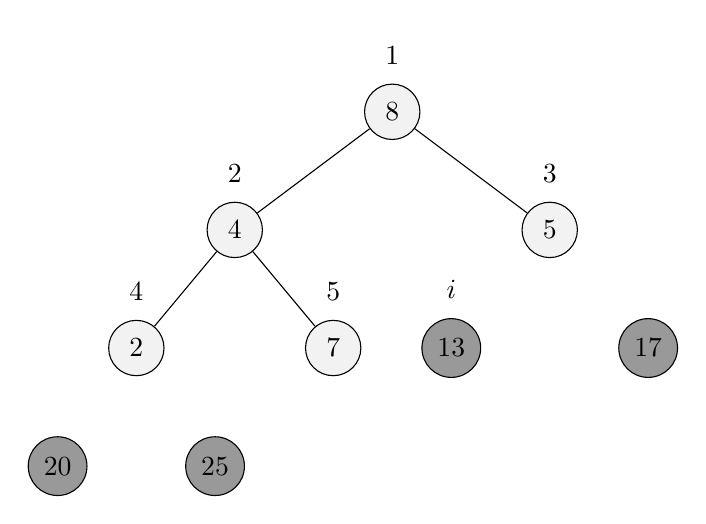
\begin{tikzpicture}
   \tikzstyle{level 1}=[sibling distance=4cm]
   \tikzstyle{level 2}=[sibling distance=2.5cm]
   \tikzstyle{level 3}=[sibling distance=2cm]
   \tikzstyle{every node}=[draw, circle, fill=gray, fill opacity=0.1, text opacity=1, minimum size=2em]
   
\node[label=90:$1$] {8}
    child {node[label=90:$2$] {4}
        child {node[label=90:$4$] {2}
            child {node[fill=black, fill opacity=0.4] {20} edge from parent[draw=none]}
            child {node[fill=black, fill opacity=0.4] {25} edge from parent[draw=none]}
        }
        child {node[label=90:$5$] {7}}
    }
    child {node[label=90:$3$] {5}
        child {node[label=90:$i$, fill=black, fill opacity=0.4] {13} edge from parent[draw=none]}
        child {node[fill=black, fill opacity=0.4] {17} edge from parent[draw=none]}
    };

\end{tikzpicture}
\end{center}

\begin{center}
    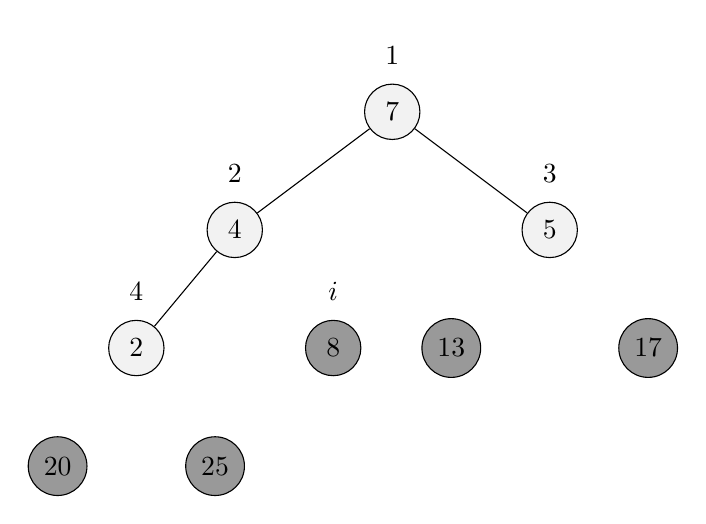
\begin{tikzpicture}
   \tikzstyle{level 1}=[sibling distance=4cm]
   \tikzstyle{level 2}=[sibling distance=2.5cm]
   \tikzstyle{level 3}=[sibling distance=2cm]
   \tikzstyle{every node}=[draw, circle, fill=gray, fill opacity=0.1, text opacity=1, minimum size=2em]
   
\node[label=90:$1$] {7}
    child {node[label=90:$2$] {4}
        child {node[label=90:$4$] {2}
            child {node[fill=black, fill opacity=0.4] {20} edge from parent[draw=none]}
            child {node[fill=black, fill opacity=0.4] {25} edge from parent[draw=none]}
        }
        child {node[label=90:$i$, fill=black, fill opacity=0.4] {8} edge from parent[draw=none]}
    }
    child {node[label=90:$3$] {5}
        child {node[fill=black, fill opacity=0.4] {13} edge from parent[draw=none]}
        child {node[fill=black, fill opacity=0.4] {17} edge from parent[draw=none]}
    };

\end{tikzpicture}
\end{center}

\begin{center}
    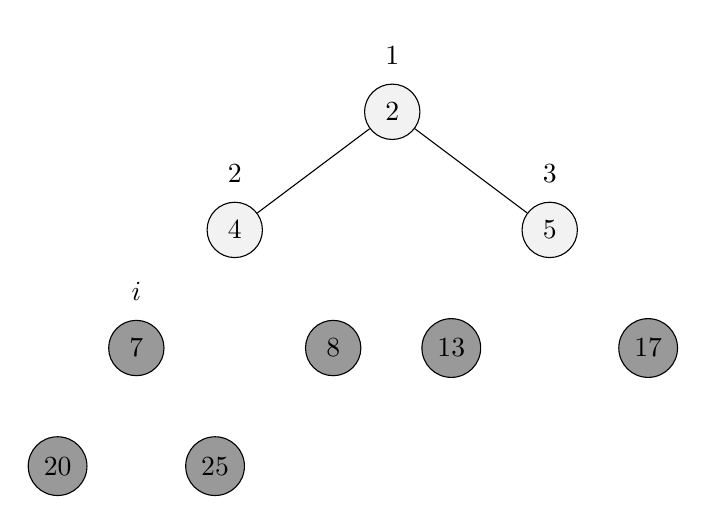
\begin{tikzpicture}
   \tikzstyle{level 1}=[sibling distance=4cm]
   \tikzstyle{level 2}=[sibling distance=2.5cm]
   \tikzstyle{level 3}=[sibling distance=2cm]
   \tikzstyle{every node}=[draw, circle, fill=gray, fill opacity=0.1, text opacity=1, minimum size=2em]
   
\node[label=90:$1$] {2}
    child {node[label=90:$2$] {4}
        child {node[label=90:$i$, fill=black, fill opacity=0.4] {7} edge from parent[draw=none]
            child {node[fill=black, fill opacity=0.4] {20} edge from parent[draw=none]}
            child {node[fill=black, fill opacity=0.4] {25} edge from parent[draw=none]}
        }
        child {node[fill=black, fill opacity=0.4] {8} edge from parent[draw=none]}
    }
    child {node[label=90:$3$] {5}
        child {node[fill=black, fill opacity=0.4] {13} edge from parent[draw=none]}
        child {node[fill=black, fill opacity=0.4] {17} edge from parent[draw=none]}
    };

\end{tikzpicture}
\end{center}

\begin{center}
    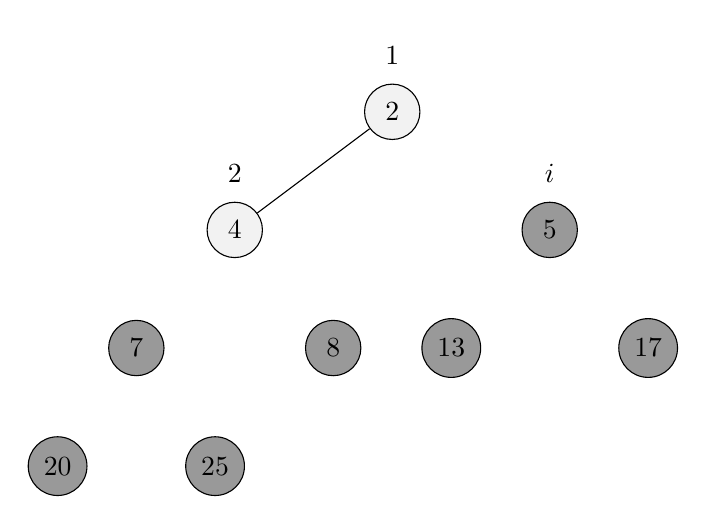
\begin{tikzpicture}
   \tikzstyle{level 1}=[sibling distance=4cm]
   \tikzstyle{level 2}=[sibling distance=2.5cm]
   \tikzstyle{level 3}=[sibling distance=2cm]
   \tikzstyle{every node}=[draw, circle, fill=gray, fill opacity=0.1, text opacity=1, minimum size=2em]
   
\node[label=90:$1$] {2}
    child {node[label=90:$2$] {4}
        child {node[fill=black, fill opacity=0.4] {7} edge from parent[draw=none]
            child {node[fill=black, fill opacity=0.4] {20} edge from parent[draw=none]}
            child {node[fill=black, fill opacity=0.4] {25} edge from parent[draw=none]}
        }
        child {node[fill=black, fill opacity=0.4] {8} edge from parent[draw=none]}
    }
    child {node[label=90:$i$, fill=black, fill opacity=0.4] {5} edge from parent[draw=none]
        child {node[fill=black, fill opacity=0.4] {13} edge from parent[draw=none]}
        child {node[fill=black, fill opacity=0.4] {17} edge from parent[draw=none]}
    };

\end{tikzpicture}
\end{center}

\begin{center}
    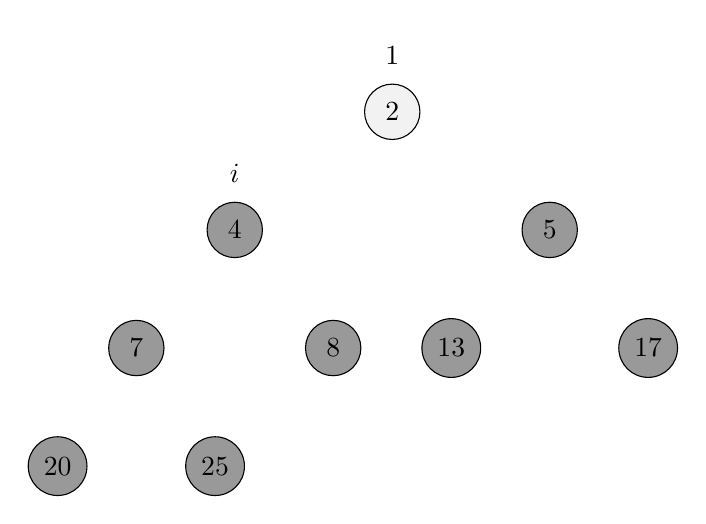
\begin{tikzpicture}
   \tikzstyle{level 1}=[sibling distance=4cm]
   \tikzstyle{level 2}=[sibling distance=2.5cm]
   \tikzstyle{level 3}=[sibling distance=2cm]
   \tikzstyle{every node}=[draw, circle, fill=gray, fill opacity=0.1, text opacity=1, minimum size=2em]
   
\node[label=90:$1$] {2}
    child {node[label=90:$i$, fill=black, fill opacity=0.4] {4} edge from parent[draw=none]
        child {node[fill=black, fill opacity=0.4] {7} edge from parent[draw=none]
            child {node[fill=black, fill opacity=0.4] {20} edge from parent[draw=none]}
            child {node[fill=black, fill opacity=0.4] {25} edge from parent[draw=none]}
        }
        child {node[fill=black, fill opacity=0.4] {8} edge from parent[draw=none]}
    }
    child {node[fill=black, fill opacity=0.4] {5} edge from parent[draw=none]
        child {node[fill=black, fill opacity=0.4] {13} edge from parent[draw=none]}
        child {node[fill=black, fill opacity=0.4] {17} edge from parent[draw=none]}
    };

\end{tikzpicture}
\end{center}

\vspace{0.5cm}

\begin{center}
    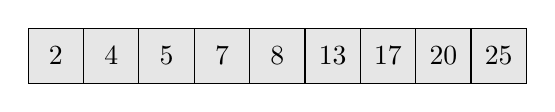
\begin{tikzpicture}[
        start chain = going right, node distance = 0pt, 
        every node/.style={draw, minimum width=2em, minimum height=2em,
                            outer sep=0pt, on chain, fill=gray, fill opacity=0.2, text opacity=1},
        ]
    \node[] {$2$};
    \node[] {$4$};
    \node[] {$5$};
    \node[] {$7$};
    \node[] {$8$};
    \node[] {$13$};
    \node[] {$17$};
    \node[] {$20$};
    \node[] {$25$};
    \end{tikzpicture}
\end{center}

\end{enumerate}

\end{document}
